\documentclass[note]{TechNote}
\usepackage[centertags]{amsmath}
\usepackage{amssymb,amsthm}
\usepackage[mathcal]{euscript}
\usepackage{tabularx}
\usepackage{cite}
\usepackage{c++}
\usepackage{tmadd,tmath}

%%---------------------------------------------------------------------------%%
\begin{document}

\refno{CSMD-00-000}
\subject{A Multilevel Monte Carlo Solver for Linear Systems}

\TIname{Mathematics and Computer Science Division}
\groupname{Computational Engineering and Energy Sciences Group}
\from{Stuart R. Slattery}
\date{\today}
\audience{
  \email{Stuart Slattery}{slatterysr@ornl.gov} \\
  \email{Tom Evans}{evanstm@ornl.gov} \\
  \email{Steven Hamilton}{hamiltonsp@ornl.gov}
}

%%---------------------------------------------------------------------------%%
\opening

\begin{abstract}
  Monte Carlo solvers for linear systems have been demonstrated to
  perform poorly for strongly elliptic problems. This poor performance
  is primarily due to the fact that both a large number of samples are
  required to obtain a good statistical error and that these samples
  require a large amount of time to compute. As a mechanism to reduce
  the computational complexity for such problems and thereby improve
  the figure of merit of the calculation, multilevel Monte Carlo has
  been introduced in finance problems, the solution of stochastic
  partial differential equations, and other algorithms that leverage
  Markov chain Monte Carlo. We adapt these ideas to form a multilevel
  Monte Carlo solver for linear systems which, in the form presented
  here, is effectively a stochastic realization of a geometric
  multigrid solver. Numerical studies indicate that the new multilevel
  method can reduce the time required to achieve a certain statistical
  error in the solution by at least two orders of magnitude, thereby
  dramatically reducing the computational complexity of the
  problem. Furthermore, the general formulation presented here
  indicates that this methodology is not restricted to geometric
  formulations of the multigrid method and could additionally be
  formulated using algebraic techniques.
\end{abstract}

%%---------------------------------------------------------------------------%%
\section{Introduction}
\label{sec:introduction}
Monte Carlo solvers for linear systems have been in existence for
decades as a stochastic alternative to iterative methods
\cite{forsythe_matrix_1950,wasow_note_1952,halton_sequential_1962,hammersley_monte_1964,spanier_monte_1969}. However,
these methods have failed to gain popularity both in the mathematics
and applications community partly due to their slow convergence bound
by the central limit theorem. Recent work has indicated that when used
as an acceleration in the Monte Carlo Synethetic Acceleration (MCSA)
method, exponential convergence rates may be achieved that are
competetive with contemporary iterative methods
\cite{evans_residual_2003,evans_monte_2009,evans_monte_2012,slattery_phd_2013}.
However, in this recent work it was discovered that for physics
problems that are largely elliptic (e.g. neutron transport in a light
water reactor), convergence of the Monte Carlo method is extremely
slow and prohibitive for the solution of larger systems. One avenue to
improve the time to solution for these calculations and to enable the
solution of more difficult problems is to study preconditioning
strategies as in \cite{slattery_phd_2013}. Another approach is to
instead focus on improving the time complexity of the Monte Carlo
sequence independent of the condition number of the linear problem.

Recent work in Monte Carlo methods for problems in finance and
stochastic partial differential equations has indicated that the
computationaly complexity of the problem can be dramatically reduced
by incorporating multigrid concepts into the solution scheme
\cite{heinrich_2001,giles_2008,cliffe_2011}. In this work, we adapt
those ideas and apply them to the Monte Carlo problem for linear
systems as a means of reducing the computational complexity of the
algorithm. To begin, we first introduce the elliptic model problem for
our numerical experiments and compare the behavior of the Monte Carlo
method to traditional iterative smoothers that would be used with the
multigrid method. Next, we present the multilevel Monte Carlo method
for linear systems using a general algebraic formulation. Finally, we
present results using the model problem the demonstrate the
superiority of the multilevel method.

%%---------------------------------------------------------------------------%%
\section{Monte Carlo Solver Fourier Analysis}
\label{sec:fourier_analysis}
The numerical analysis presented here closely follows that presented
in \cite{briggs_multigrid} for multigrid problems. For this analysis,
we will use the following one-dimensional, homogenous model problem:
\begin{equation}
  \nabla^2 x = 0\:.
  \label{eq:model_problem}
\end{equation}
We discretize the problem into $N$ discrete points
where now $\ve{x} \in \mathbb{R}^N$ with boundary conditions:
\begin{equation}
  \ve{x}_1 = 0,\ \ \ve{x}_N = 0\:.
  \label{eq:boundary_conditions}
\end{equation}
The Laplacian is discretized using a standard second-order finite
difference with a grid spacing of one:
\begin{equation}
  (\nabla \ve{u})_i = \ve{u}_{i-1} - 2 \ve{u}_{i} + \ve{u}_{i+1}\:,
  \label{eq:discrete_laplacian}
\end{equation}
which then gives the following linear problem:
\begin{equation}
  \ve{A}\ve{x} = \ve{0}\:.
  \label{eq:linear_problem}
\end{equation}
To bound the spectral radius of the problem we will use a Jacobi
preconditioner:
\begin{equation}
  \ve{M} = diag(\ve{A})\:,
  \label{eq:preconditioner}
\end{equation}
such that we instead solve the following linear problem:
\begin{equation}
  \ve{M}^{-1}\ve{A}\ve{x} = \ve{0}\:.
  \label{eq:precond_problem}
\end{equation}

To elucidate the effect of a given solution technique on a given error
mode in the problem, we can assign an initial guess of $\ve{x}^0$ to
be a chosen Fourier mode:
\begin{equation}
  \ve{x}^0_i = \sin\Bigg( \frac{ik\pi}{N} \Bigg)\:,
  \label{eq:fourier_mode}
\end{equation}
where $\ve{x}^0_i$ is the $i^{th}$ component of the initial guess and
k is the wave number of the chosen Fourier mode. First, we will look at
the performance Richardson's iteration as the smoother which is
equivalently a Jacobi iteration when Jacobi preconditioning is used:
\begin{equation}
  \ve{x}^{k+1} = (\ve{I}-\ve{M}^{-1}\ve{A})\ve{x}^k\:,
\end{equation}
where $k$ is the iteration index. Figure~\ref{fig:richardson} gives
infinity norm of the error in the solution vector\footnote{The
  solution to the homogenous problem is zero and therefore
  $||\ve{e}||_{\infty} = ||\ve{x}||_{\infty}$} as a function of
iterations for wave numbers of 1, 5, and 10 on a grid with N = 100.
\begin{figure}[h!]
  \begin{center}
    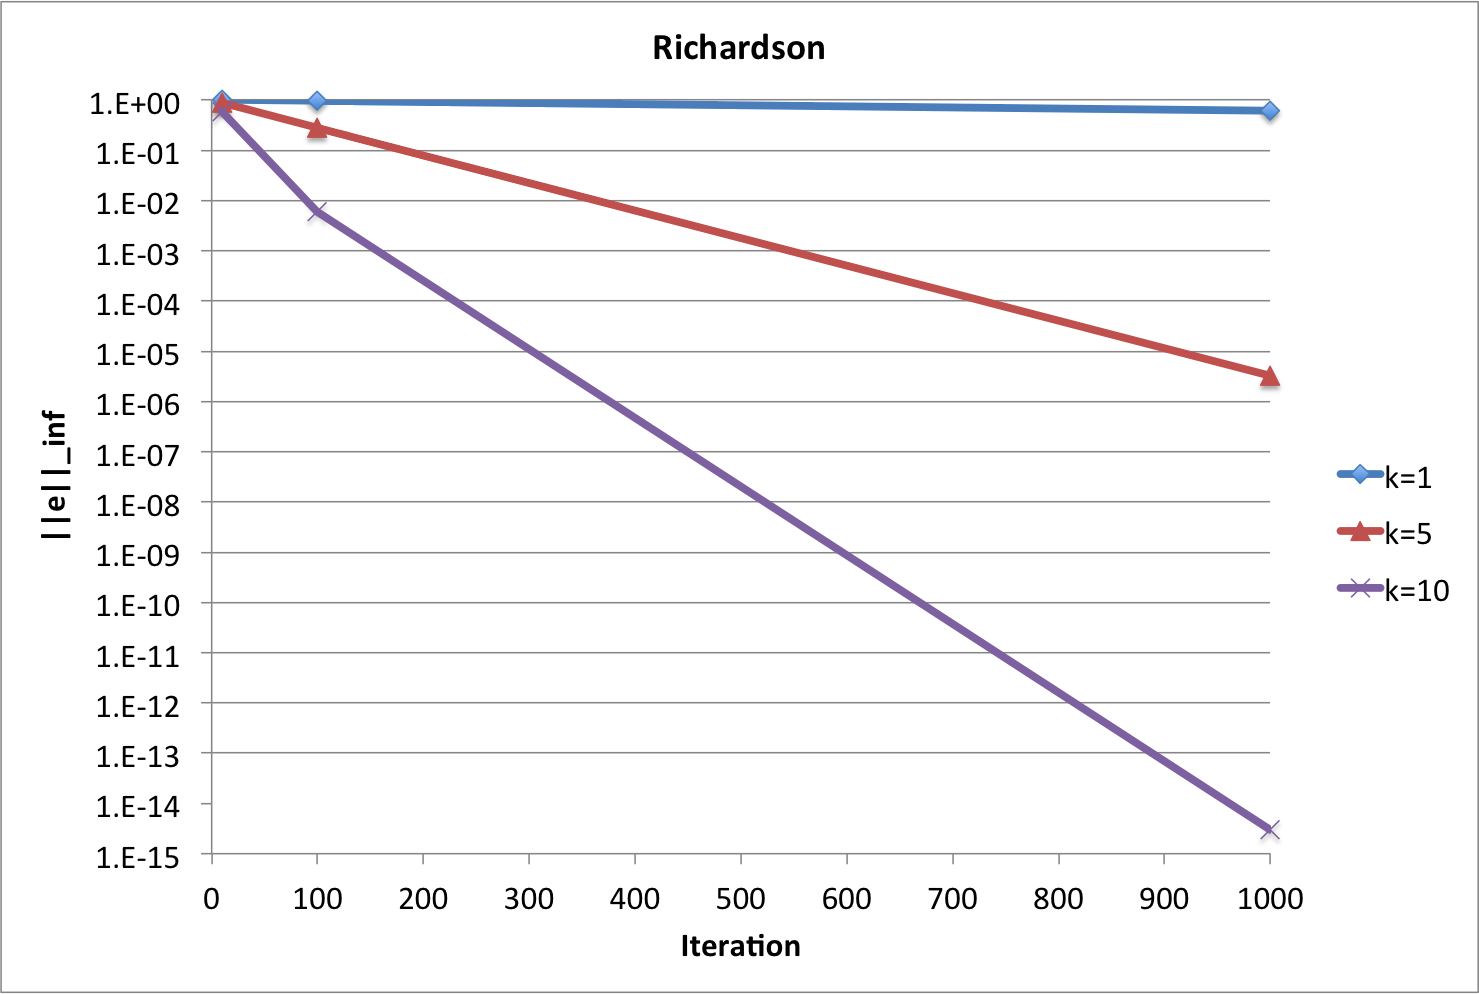
\includegraphics[width=5in]{richardson.png}
  \end{center}
  \caption{\textbf{Convergence of Richardson's iteration as a function
      of iteration for a grid of size N = 100.} \textit{Richardson's
      iteration performs better for larger wave numbers and therefore
      more oscillatory modes.}}
  \label{fig:richardson}
\end{figure}
Immediately we note that the larger the wave number the better
Richardson's iteration performs. Per the spectral analysis in
\cite{briggs_multigrid}, this iteration sequence perfoms better for
higher wave numbers as the eigenvalue spectrum spans a smaller space
then less oscillatory modes. This behavior motivated the multigrid
approach where moving a smooth mode to a coarser grid makes that mode
appear more oscillatory relative to that coarser grid, thus improving
convergence for that particular mode.

Next we perform the same calculations using the adjoint Monte Carlo
solver presented in \cite{evans_monte_2012}. Before doing this
however, we must first modify the linear problem as the Monte Carlo
solver is a direct method and therefore a homogenous problem with a
right hand side of $\ve{0}$ will yield no samples. Instead, we will
solve the residual problem:
\begin{equation}
  \ve{A}\ve{d} = \ve{r}\:,
  \label{eq:residual_problem}
\end{equation}
where the residual of the homogenous problem is:
\begin{equation}
  \ve{r} = -\ve{A}\ve{x}^0\:,
  \label{eq:homogenous_residual}
\end{equation}
and the solution is computed as:
\begin{equation}
  \ve{x} = \ve{x}^0 + \ve{d}\:.
  \label{eq:residual_solution}
\end{equation}
Forming the problem in this way lets us directly apply the adjoint
Monte Carlo method to the homogenous problem and then apply the
effective correction, $\ve{d}$, to the initial guess to give the
solution. This approach is also equivalent to performing a single
iteration of Halton's method \cite{halton_sequential_1962}. Using this
formulation we can again solve the model problem with wave numbers of
1, 5 and 10 on a grid of size N=1 but this time we vary the number of
histories used to compute the solution instead of the number of
iterations. Figure~\ref{fig:adjoint_mc} gives the results of this
calculation.
\begin{figure}[h!]
  \begin{center}
    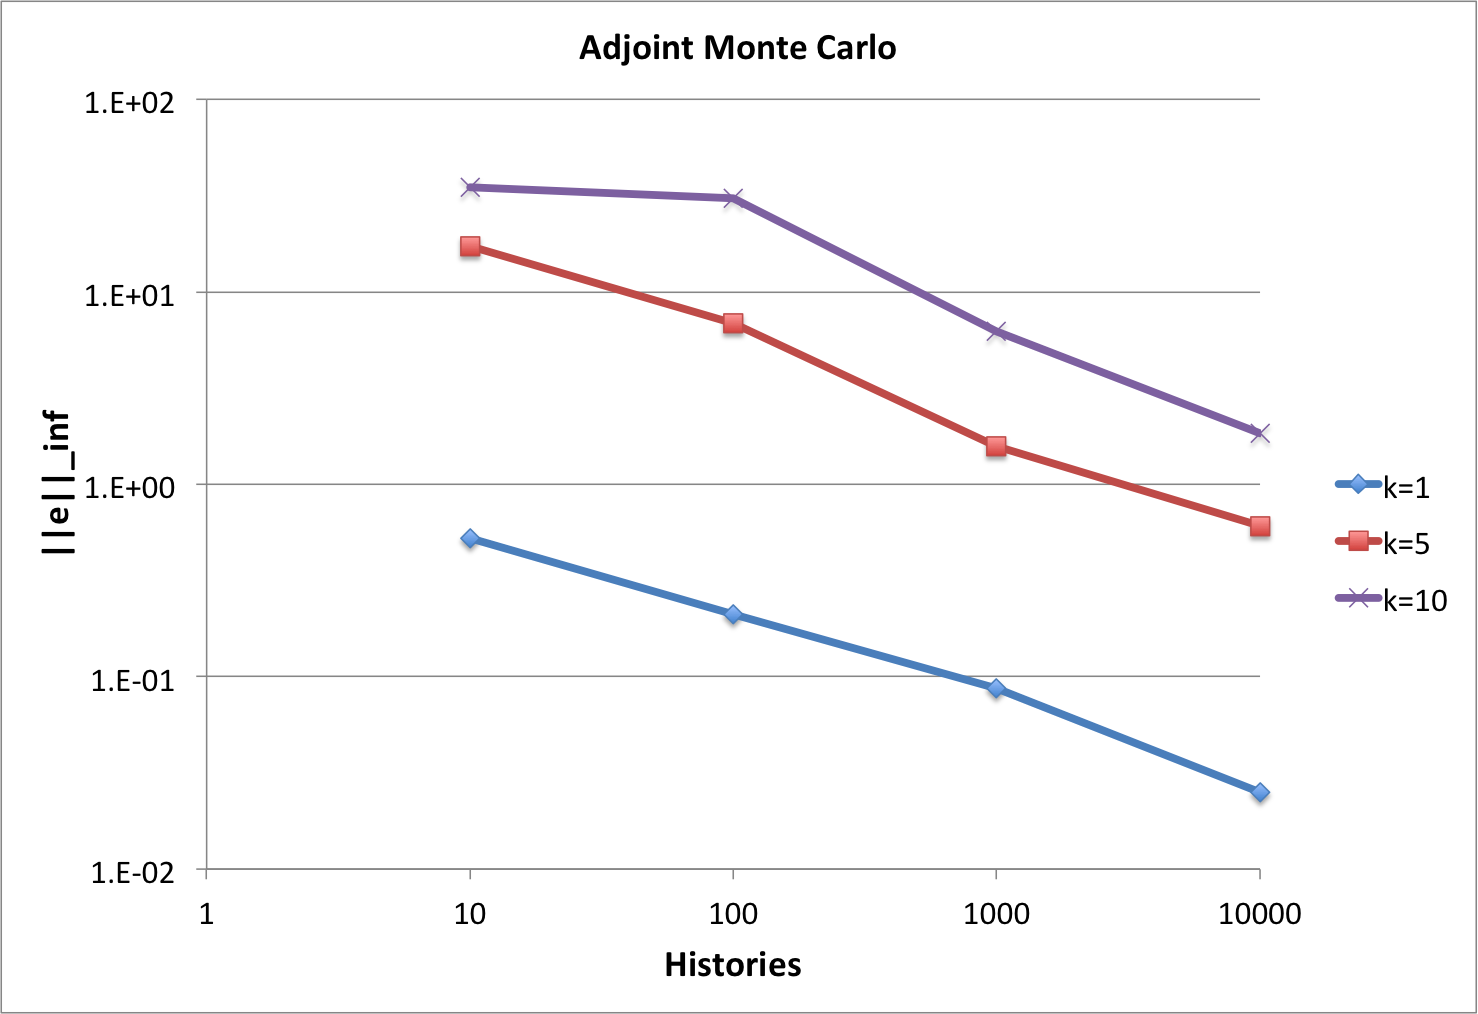
\includegraphics[width=5in]{adjoint_mc.png}
  \end{center}
  \caption{\textbf{Convergence of the adjoint Monte Carlo method as a
      function of sampled histories for a grid of size N = 100.}
    \textit{Adjoint Monte Carlo performs better for smaller wave
      numbers and therefore smoother modes.}}
  \label{fig:adjoint_mc}
\end{figure}
Surprisingly, the Monte Carlo method performs better for smooth modes
then more oscillatory modes\footnote{This behavior was also observed
  for the forward Monte Carlo method presented in
  \cite{evans_monte_2012}}. The results of these calculations are
counterintuitive given the fact that the Monte Carlo solver is
effectively a stochastic realization of of Richardson's iteration and
therefore one should expect the same spectral behavior from the
results. 

Looking at the timing results in Table~\ref{tab:mc_timing}, we see
that the behavior of the Monte Carlo solver is in fact consistent with
expectations.
\begin{table}[h!]
  \begin{center}
    \begin{tabular}{cc}\hline\hline
      \multicolumn{1}{c}{\textbf{Wave Number}} & 
      \multicolumn{1}{c}{\textbf{Time per History (s)}} \\
      \hline
      1 & 1 \\
      5 & 0.85 \\
      10 & 0.83 \\
      \hline\hline
    \end{tabular}
  \end{center}
  \caption{\textbf{Normalized average CPU time per history.}}
  \label{tab:mc_timing}
\end{table}
Timing results show that the average time required to compute an
entire history in the Monte Carlo solver decreases as a function of
wave number. We showed analytically in \cite{slattery_2013} that the
length of the random walk is equivalent to the number of Richardson
iterations that would be required to achieve a given convergence
criteria. In Figure~\ref{fig:richardson}, we see that fewer iterations
are required to converge larger wave numbers and therefore we should
also expect shorter random walks in the Monte Carlo solver and
therefore a faster time to solution as observed in
Table~\ref{tab:mc_timing}.

%%---------------------------------------------------------------------------%%
\section{Multilevel Monte Carlo Algorithm}
\label{sec:algorithm}

%%---------------------------------------------------------------------------%%
\section{Results}
\label{sec:results}

%%---------------------------------------------------------------------------%%
\bibliographystyle{ieeetr}
\bibliography{references}

\closing
\caution
\end{document}
